69. \begin{figure}[ht!]
\center{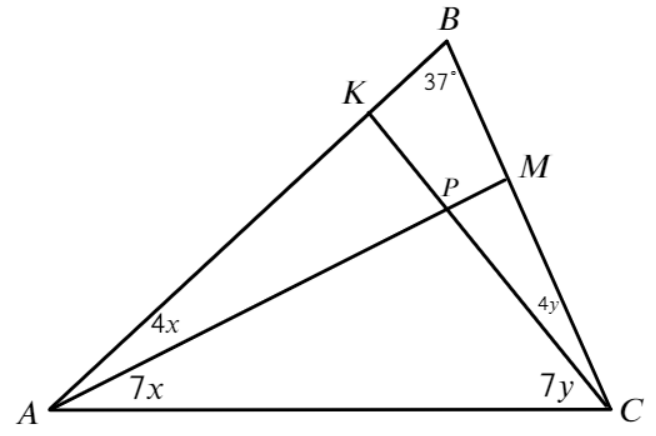
\includegraphics[scale=0.35]{g69.png}}
\end{figure}\\
Обозначим $\angle BAM=4x,\ \angle CAM=7x,\ \angle BCK=4y,\ \angle ACK=7y.$ Тогда из треугольника $ABC:\ 4x+7x+4y+7y+37^\circ=180^\circ,\ 11(x+y)=143^\circ,\ x+y=13^\circ.$ Теперь запишем сумму углов треугольника $APC:\ 7x+7y+\angle APC=180^\circ,\ \angle APC=180^\circ-7(x+y)=180^\circ-7\cdot13^\circ=89^\circ.$\\
